\section{Background Research}

\subsection{Object Detection}

We must select appropriate algorithms for surgical tool detection and compare them using various meaningful metrics. Algorithms must have faster inference times in clinical contexts on sufficiently fast hardware to enable real-time execution \cite{ali2023comprehensivesurveyrecentdeep}. Their architectures and complexity must also differ enough to draw meaningful conclusions. With an abundance of models to choose from, we pick a set of state-of-the-art (SOTA) models with characteristics suitable for further analysis.

\subsubsection{Anchor-Boxes}

Anchor boxes are predefined bounding boxes of various aspect ratios and scales used in object detection models to predict the locations of objects within an image \cite{Zhong_2020_WACV, wang_region_2019}. In anchor-based models, non-maximum suppression (NMS) often eliminates duplicate detections, reducing false positives \cite{redmon_you_2016}. In the surgical context, tools vary significantly in size, aspect ratio, and orientation and can move dynamically across the entire image. Using anchor boxes allows models to effectively predict bounding boxes that match these tools' diverse shapes and movements. However, the fixed nature of anchor boxes can sometimes limit the model's flexibility, particularly when tools exhibit unusual rotations or positions that fall outside the predefined anchor aspect ratios and configurations. This limitation suggests that anchor-free models not relying on predefined boxes may offer greater adaptability in complex scenarios. 
% Nonetheless, to ensure a thorough evaluation, especially as anchor-based comparisons are lacking in in-vitro contexts, we aim to compare anchor-based and anchor-free methods to determine which approach performs best in detecting and tracking surgical tools under these challenging conditions.

\subsubsection{State-of-the-Art Models}

YOLOv8 \cite{jocher_ultralytics_2023}, an iteration of the well-known You-Only-Look-Once (YOLO) models, is an anchor-free model known for its efficiency and speed, utilising a convolutional neural network (CNN) architecture that is particularly well-suited for real-time surgical tool detection and tracking based on ample previous work with earlier YOLO models \cite{raja_performance_2024, redmon_you_2016, yolo7_2024, wang_visual_2022, cho_automatic_2021, choi_surgical-tools_2017, jo_robust_2019, benavides_real-time_2024}. As a lightweight model, it can achieve high accuracy in detecting laparoscopic tools while being faster in RCEs due to its lower complexity \cite{yolo7_2024}. YOLOv10, an evolution of the YOLO series, introduces NMS-free training, maintaining its anchor-based nature \cite{ultralytics_yolov10_2024}. It frames object detection as a regression problem by minimising the error in bounding boxes and optimising the end-to-end detection pipeline. YOLO models have shown fast convergence in training and a wide range of adaptability across various domains. They use mosaic augmentation to improve generalisation, where images are cropped and stitched together, increasing the model's robustness to different spatial contexts. Multiple varying architectural sizes for both YOLOs exist, which we will evaluate to see the effects of model complexity.

EfficientDet \cite{tan_efficientdet_2019} is an anchor-based method which employs a CNN architecture with a compound scaling approach to balance accuracy and efficiency, making it particularly effective for RCEs. RetinaNet \cite{zlocha_improving_2019}, based on the ResNet backbone \cite{he_deep_2015}, leverages focal loss \cite{lin_focal_2017} to handle class imbalance, making it a robust choice for detection, where some classes may dominate the dataset. RetinaNet's anchor box optimisation further enhances its precision, and additional improvements have been proposed to optimise it further for surgical contexts, which can allow it to outperform other anchor-based methods \cite{zlocha_martinzlochaanchor-optimization_2024}. DETR (DEtection TRansformer) utilises a transformer-based architecture that redefines object detection as a direct set prediction problem, eliminating the need for hand-designed components like NMS and anchor generation \cite{10.1007/978-3-030-58452-8_13}. While DETR can be computationally intensive, it offers a streamlined detection pipeline that is particularly advantageous for complex surgical environments. We focus on the standard DETR model, although improved versions with multi-scale features and contrastive learning exist \cite{loza_realtime_2024}. SIMO, an anchor-free model, is designed for multi-output tasks, simplifying the detection process while maintaining high accuracy across various surgical scenarios. By focusing on tool and tip detection, SIMO efficiently handles the complexities of multi-object tracking \cite{hasan_detection_2021}.

% The field of surgical tool detection and tracking has seen significant advancements with the advent of deep learning and computer vision technologies. Existing models such as RetinaNet, EfficientDet, YOLOv8, YOLOv10, ART-Net, and DTX have demonstrated varying degrees of success in detecting and tracking surgical instruments in real-time, which is crucial for applications in MIS. These models leverage sophisticated architectures, including convolutional neural networks (CNNs) and time-series analysis, to accurately identify and locate surgical tools within video frames. The anchor-based models, such as those built on the YOLO architecture, use predefined anchor boxes to predict bounding boxes, while anchor-free models like ART-Net predict the location of tools directly, potentially offering greater flexibility in varying surgical environments. The evaluation of these models is commonly performed using the Common Objects in Context (COCO) dataset's metrics, particularly the mean Average Precision (mAP) and Intersection over Union (IoU) scores, which provide a robust measure of the model's performance in detecting objects within a defined area. 
% % https://ietresearch.onlinelibrary.wiley.com/action/getFTRLinkout?url=http%3A%2F%2Fscholar.google.com%2Fscholar_lookup%3Fhl%3Den%26publication_year%3D2018%26author%3DA.%2BJin%26author%3DS.%2BYeung%26author%3DJ.%2BJopling%26author%3DJ.%2BKrause%26title%3DTool%2Bdetection%2Band%2Boperative%2Bskill%2Bassessment%2Bin%2Bsurgical%2Bvideos%2Busing%2Bregion%25E2%2580%2590based%2Bconvolutional%2Bneural%2Bnetworks&doi=10.1049%2Fhtl2.12060&linkType=gs&linkLocation=Reference&linkSource=FULL_TEXT, 
% % https://doi.org/10.1109/ACCESS.2020.2969885
% % https://doi.org/10.1080/21681163.2022.2150688

% We will not discuss the exact performance of these models nor compare them against each other directly here as there are various context and different metrics used. We will have further discussions on this later in the paper.

% Even though there are works in surgical tool detection in literature, these methods are widely built on anchor-based methods, do not incorporate multi-scale feature embedding for tackling variable tool sizes, and suffer from low speed

% % \subsubsection{You Only Look Once (YOLO)}

% YOLOv10 has various modifications and improvements compared to previous versions, reducing latency and improving accuracy \cite{ultralytics_yolov10_2024}. 

% frame object detection as a regression problem to spatially separated bounding boxes and associated class probabilities. A single neural network predicts bounding boxes and class probabilities directly from full images in one evaluation. Since the whole detection pipeline is a single network, it can be optimized end-to-end directly on detection performance. YOLO learns very general representations of objects. A single convolutional network simultaneously predicts multiple bounding boxes and class probabilities for those boxes. YOLO trains on full images and directly optimizes detection performance. This unified model has several benefits over traditional methods of object detection. Unlike classifier-based approaches, YOLO is trained on a loss function that directly corresponds to detection performance and the entire model is trained jointly. YOLO also generalizes well to new domains making it ideal for applications that rely on fast, robust object detection. 
% % https://arxiv.org/abs/1506.02640
% YOLO: Redmon et al.[19] proposed YOLO (You Only Look Once) algorithm in 2016. As the earliest one-stage detection algorithm, it treats the object detection task as a regression problem, and predicts the coordinates of the bounding box, the categories of objects contained in the bounding box and the confidence of classification by directly processing the whole image. 
% % https://www.sciencedirect.com/science/article/pii/S0921889021002232
% % https://d197for5662m48.cloudfront.net/documents/publicationstatus/182926/preprint_pdf/c01200a120dadb10c17594a11edcded8.pdf 

% Anchor-based is interesting because videos often have a wide range of aspect ratios, etc. (insert examples). We decided that it would be best to continue with the current dataset, and to make it scientific and sufficient for the MSc, I would look at investigating anchor-based methods (e.g. YOLO) and anchor-less methods (fully connected one-stage CNN). A method for each would be sufficient. The idea is that the aspect ratio of the tool will change as it moves around and is rotated, with different orientations and scales in various ways, so anchors in anchor-based methods would need to be optimised. I would look at what methods could cope with those situations and what their limitations are.

% Non-maximum suppression (NMS) is a technique used in object detection to remove overlapping bounding boxes. It is a post-processing algorithm that filters out boxes with low confidence scores and high IoU (Intersection over Union) with other boxes. NMS is a crucial step in object detection pipelines to ensure that the model predicts only one bounding box for each object. The algorithm works by selecting the box with the highest confidence score and removing all other boxes that have a high IoU with the selected box. This process is repeated until all boxes are processed. NMS is an essential step in object detection pipelines to ensure that the model predicts accurate bounding boxes for objects in the image. 
% % https://www.pyimagesearch.com/2020/08/10/opencv-object-tracking/

% The execution time of NMS primarily depends on the number of boxes and two thresholds. As the confidence threshold increases, more prediction boxes are filtered out, and the number of remaining boxes that need to calculate IoU decreases, thus reducing the execution time of NMS. Another observation is that anchor-free detectors outperform anchor-based detectors with equivalent accuracy for YOLO detectors because the former require less NMS time than the latter.

% YOLOv10: YOLOs have emerged as the predominant paradigm in the field of real-time object detection owing to their effective balance between computational cost and detection performance. Researchers have explored the architectural designs, optimization objectives, data augmentation strategies, and others for YOLOs, achieving notable progress. consistent dual assignments for NMS-free training of YOLOs, which brings the competitive performance and low inference latency simultaneously. Moreover, we introduce the holistic efficiency-accuracy driven model design strategy for YOLOs. We comprehensively optimize various components of YOLOs from both the efficiency and accuracy perspectives, which greatly reduces the computational overhead and enhances the capability achieves the stateof-the-art performance and efficiency across various model scales.
% we target both the post-processing and model architecture throughout the detection pipeline of YOLOs. For the post-processing, we propose the consistent dual assignments for NMSfree training, achieving efficient end-to-end detection. For the model architecture, we introduce the holistic efficiency-accuracy driven model design strategy, improving the performance-efficiency tradeoffs. These bring our YOLOv10, a new real-time end-to-end object detector. Extensive experiments show that YOLOv10 achieves the state-of-the-art performance and latency compared with other advanced detectors, well demonstrating its superiority. 
% % https://arxiv.org/pdf/2405.14458

% A YOLO-based model was presented by Choi et al. [20]. His work reported the fastest inference time of 48 FPS in the m2cai16-tool-location dataset but low performance for localization over preselected videos for validation. 
% % Choi, B., Jo, K., Choi, S., Choi, J.: Surgical-tools detection based on convolutional neural network in laparoscopic robot-assisted surgery. In: Proceedings of the Annual International Conference of the IEEE Engineering in Medicine and Biology Society, EMBS, pp.  1756–1759. IEEE, Piscataway, NJ (2017)

% "We trained two state-of-the-art detectors, RetinaNet and YOLOv2, with bounding boxes centered around the tip annotations with specific margin sizes to determine the optimal margin size for detecting the tip of the instrument and localising the point. 
% % https://www.sciencedirect.com/science/article/pii/S0010482521001785

% https://ietresearch.onlinelibrary.wiley.com/doi/full/10.1049/htl2.12072 looked at "This study focuses on enhancing the inference speed of laparoscopic tool detection on embedded devices. Laparoscopy, a minimally invasive surgery technique, markedly reduces patient recovery times and postoperative complications. Real-time laparoscopic tool detection helps assisting laparoscopy by providing information for surgical navigation, and its implementation on embedded devices is gaining interest due to the portability, network independence and scalability of the devices. However, embedded devices often face computation resource limitations, potentially hindering inference speed. To mitigate this concern, the work introduces a two-fold modification to the YOLOv7 model: the feature channels and integrate RepBlock is halved, yielding the YOLOv7-RepFPN model. This configuration leads to a significant reduction in computational complexity. Additionally, the focal EIoU (efficient intersection of union) loss function is employed for bounding box regression. Experimental results on an embedded device demonstrate that for frame-by-frame laparoscopic tool detection, the proposed YOLOv7-RepFPN achieved an mAP of 88.2\% (with IoU set to 0.5) on a custom dataset based on EndoVis17, and an inference speed of 62.9 FPS. Contrasting with the original YOLOv7, which garnered an 89.3\% mAP and 41.8 FPS under identical conditions, the methodology enhances the speed by 21.1 FPS while maintaining detection accuracy. This emphasizes the effectiveness of the work. A detection speed of 25–30 FPS is generally seen as real-time [10, 11]."

% % https://www.mdpi.com/2076-3417/9/14/2865 
% Firstly, the proposed method can detect surgical tools in real time by using the object detection system YOLO9000. Unlike other methods, You Only Look Once (YOLO) does not allow for finding the region of interest (ROI). Conventional methods aim to identify the ROI from an input image and thereafter, to classify each ROI. However, applying YOLO allowed for the diminishing of the time required to calculate the ROI. YOLO divides an input image into a set of grid cells and then, performs classification of each grid cell. Owing to this key feature of YOLO, the proposed algorithm can detect surgical tools in real time (Table 3).

% % https://d197for5662m48.cloudfront.net/documents/publicationstatus/182926/preprint_pdf/c01200a120dadb10c17594a11edcded8.pdf 
% We found that the performance of all the NAS-based YOLO was inferior as compared to other State-of-the-Art (SoTA) YOLO models. We compare our results against the YOLOv7 model too.

% % https://www.mdpi.com/1424-8220/24/13/4191 
% "The You Only Look Once (YOLO) algorithm [15] implements this unified approach by framing object detection as a regression problem. YOLO is recognized as one of the most efficient algorithms, suitable for real-time processing, due to its single convolutional network evaluation. The YOLO architecture was introduced by Choi et al. [16] for real-time surgical instrument tracking. They achieved 72.26\% mean average precision on a dataset that included seven surgical tools. The convolutional layers were pretrained using the ImageNet 1000-class competition dataset, and then a gallbladder surgery image dataset was used for the learning process. Choi et al. finally concluded that the low precision in the detection of some specific instruments was due to the insufficient number of images to learn from. Although single-stage detectors such as YOLO show more efficiency than their twostage counterparts, both approaches rely on anchor boxes. These anchor boxes introduce numerous hyperparameters that require fine-tuning, hindering the network training process. Despite their high accuracy in surgical tool detection, methods utilising anchor boxes often fall short in real-time applications. To address this limitation, Liu et al. [17] combined an anchor-box-free CNN with an Hourglass network [18], facilitating real-time surgical tool localization through heatmap estimation. Models based on U-Net architectures [19], widely popular in segmentation tasks, have also been used to determine the position of surgical instruments [20,21]. Kurmann et al. proposed a U-shaped network to simultaneously recognize multiple instruments and their parts [22]. Laina et al. [23] formulated the position estimation task as heatmap regression, estimated concurrently with tool segmentation."

% % https://ieeexplore.ieee.org/abstract/document/10168997 
% Several approaches have been developed to achieve bounding box tool classification. One interesting implementation examined the performance of a You Only Look Once (YOLO) based network [5] across 7 different types of tools [6]. YOLO based networks boast very high performance speeds, making them an ideal choice for real time applications. However, with the lack of optimisation, they underperform in harsh environments such as the ones associated to laparoscopic or orthopaedic operations. To address this, a YOLO900 based network [7] was constructed to take into account motion prediction from previous frames in order to improve detection performance [8]. This use of temporal information, however, can lead to an exponentially increasing error, since the success of tool detection in the current frame depends on the success of previous detections. Nevertheless, this approach further underlines the high speed and tunability of YOLO based networks. These networks, however, are not the only ones that demonstrate high detection speeds. It has been shown that it is possible to achieve extremely fast box detection by constructing non-region-based networks for tool detection. Specifically, the Extremely Fast and Precise Network (EF- PNet) [9] was constructed with the aim of optimising detection speed, achieving 270 fps in detection. This research suggests that in a surgical context, YOLO based networks may not be optimal for box detection. A similar process was explored when developing a box detection network that did not require the formulation of anchors [10]. Even though the inference speed only ran at 37 fps, the accuracy was increased significantly. Another advantage of deep learning approaches was the option to integrate spatio-temporal data across the detection process to improve results. A Spatial Transformer Network (STN) has been combined with a CNN to detect tools moving at high speed, a condition which usually suffers from erroneous detections due to image blur [11]. However, occlusions significantly impact such methods.

% % \subsubsection{ART-Net Model}

% ART-Net: Problem is the model was built for segmentation. To convert this into a detection problem would significantly reduce the accuracy of the model. Though we can easily convert segmentation masks into bounding box annotations for the ART-Net dataset, annotating our dataset to be used for segmentation would be very time-consuming and not relevant as discussed in the introduction.
% ART-Net achieves in both average precision and accuracy. In segmentation, it achieves in mean Intersection over Union (mIoU) on the robotic EndoVis dataset (articulated tool), \cite{hasan_detection_2021}. The proposed framework outperforms existing ones in detection and segmentation. Compared to separate networks, integrating the tasks in a single network preserves accuracy in detection and segmentation but substantially improves accuracy in geometric primitive extraction. 
% ART-Net has a single encoder and five sub-network branches, namely one for tool detection, one for tool segmentation, and three for geometric primitive extraction.

% They achieve 100\% in detection. However, this is regarding the presence of tools, not specific instance detection with bounding boxes.

% developed a CNN they called ART-Net, for Augmented Reality Tool Network, and combined it with an algebraic geometry approach for generic tool detection, segmentation, and 3D pose estimation. While the CNN ART-Net was used for surgical tool detection and segmentation, geometric primitives were also extracted to compute the 3D pose with algebraic geometry.

% % \subsubsection{RetinaNet}

% RetinaNet: Retina-net [21] is the latest one-stage detection framework, which puts forward focus loss for unbalanced categories. It inhibits the categories with more and easier classification in the loss function and greatly improves the proportion of losses with less and difficult classification. This network structure has significant advantages in accuracy, efficiency and complexity. https://www.sciencedirect.com/science/article/pii/S0921889021002232
% % Based on ResNet He, K., Zhang, X., Ren, S., Sun, J.: Deep residual learning for image recognition. In: CVPR (2016) https://arxiv.org/abs/1512.03385

% We can use RetinaNet with anchor-box optimisation \cite{zlocha2019improving}.

% % \subsubsection{EfficientDet}

% % \subsubsection{DEtection TRansformer (DETR)}

% DETR: views object detection as a direct set prediction problem. \cite{vedaldi_end--end_2020}. streamlines the detection pipeline, effectively removing the need for many hand-designed components like a non-maximum suppression procedure or anchor generation that explicitly encode our prior knowledge about the task.
% Many Deep Learning based methods such as Fast-RCNN have achieved SOTA performance in tool detection and localization (Du et al, 2018a) but are computationally expensive, introducing inference time penalties. https://arxiv.org/abs/2209.01435.
% The goal of object detection is to predict a set of bounding boxes and category labels for each object of interest. Modern detectors address this set prediction task in an indirect way, by defining surrogate regression and classification problems on a large set of proposals [37,5], anchors [23], or window centers [53,46].
% % 23: Lin, T.Y., Goyal, P., Girshick, R.B., He, K., Doll´ar, P.: Focal loss for dense object detection. In: ICCV (2017) https://arxiv.org/abs/1708.02002v2
% % 37: Ren, S., He, K., Girshick, R.B., Sun, J.: Faster R-CNN: Towards real-time object detection with region proposal networks. PAMI (2015)
% % 5: Cai, Z., Vasconcelos, N.: Cascade R-CNN: High quality object detection and instance segmentation. PAMI (2019)
% % 53. Zhou, X., Wang, D., Kr¨ahenb¨uhl, P.: Objects as points. arXiv:1904.07850 (2019)
% % 46. Tian, Z., Shen, C., Chen, H., He, T.: FCOS: Fully convolutional one-stage object detection. In: ICCV (2019)
% DETR directly predicts (in parallel) the final set of detections by combining a common CNN with a transformer architecture [47]. During training, bipartite matching uniquely assigns predictions with ground truth boxes. 
% % 47:. Vaswani, A., Shazeer, N., Parmar, N., Uszkoreit, J., Jones, L., Gomez, A.N., Kaiser, L., Polosukhin, I.: Attention is all you need. In: NeurIPS (2017)
% DETR uses a conventional CNN backbone to learn a 2D representation of an input image. The model flattens it and supplements it with a positional encoding before passing it into a transformer encoder. A transformer decoder then inputs a small fixed number of learned positional embeddings, which we call object queries, and additionally attends to the encoder output. We pass each output embedding of the decoder to a shared feed-forward network (FFN) that predicts either a detection (class and bounding box) or a “no object” class.
% Achieves competitive results compared to Faster R-CNN in quantitative evaluation on COCO.
% % resnet backbone https://arxiv.org/abs/1512.03385

% Loza: we use advancements in \cite{Loza2023DTx}. The proposal is to utilize multi-scale features within the feature extraction layer and at the transformer-based detection architecture through positional encoding that can refine and capture context-aware and structural information of different-sized tools. Furthermore, a supervised contrastive loss is introduced to optimized representations of object embeddings, resulting in improved feed-forward network performance for classifying localized bounding boxes. The strategy demonstrates superiority to state-of-the-art (SOTA) methods. The generation of richer features is achieved by incorporating aRes2Net 
% % [https://doi.org/10.1109/TPAMI.2019.2938758] 
% as the backbone, an architecture that makes local-scale considerations for extracting features.Multi-scale position encoding of two projected feature maps extracted from the backbone to incorporate features at multiple scales in the self-attention mechanism of the transformer. We call this new architecture our proposed “dense trans-former” (DTX) network, and it is inspired by the DETRdetector \cite{vedaldi_end--end_2020}. Contrastive learning over the object representation of the surgical tools to encourage consistency and separability in the feature embeddings of the different classes

\subsection{Surgical Tool Tracking}

% Surgical tool tracking is crucial in computer-assisted surgical systems, providing insights for a range of applications, including skill assessment [1], visual surveying [2], navigation [3], laparoscope positioning [4], safety and risk zone estimation [5], and augmented reality [6, SurgiTrack]. 
% Nwoye described how traditional approaches relied on features such as colour, texture, SIFT, and geometry [7, 8, 9, 10, 11], and recent deep learning approaches have enabled more robust feature extraction for tool re-identification (re-ID), advancing the field significantly [12, 13, 14, 15, 16, 17, 18, 19, 20, 21] \cite{SurgiTrack}.
While tool detection identifies tools within a frame, tool tracking extends this by predicting the tools' locations in subsequent frames \cite{SurgiTrack}. Whilst traditional approaches relied on features such as colour, texture and geometry, recent deep learning approaches have enabled more robust feature extraction for tool re-identification (re-ID), advancing the field significantly \cite{bouget_vision-based_2017, SurgiTrack}. Despite this progress, challenges remain, particularly in multi-class tracking \cite{nwoye_2019, nwoye:tel-03855189}. Current methods primarily rely on tracking-by-detection, training a classifier to separate the region of interest from the background and then update it with new information in each frame \cite{ali2023comprehensivesurveyrecentdeep}, treating each frame as a separate detection problem, neglecting temporal continuity \cite{paley_crowdsourced_2021}. Separate frame-level labels should be used to detect tools and tips \cite{ali2023comprehensivesurveyrecentdeep}, but acquiring a large amount of such data is challenging \cite{bodenstedt_comparative_2018}. YOLO uses SOTA tracking algorithms as its default trackers: ByteTrack \cite{ByteTrack}, which associated high-confidence detections with existing tracks and retained low-confidence detections as potential new tracks, enhancing the robustness in complex scenes; and Bot-SORT \cite{BoT-SORT}, which incorporated re-ID features with strong appearance modelling, resulting in more accurate and consistent multi-object tracking.
% ...challenging \cite{bodenstedt_comparative_2018}. While this approach is advantageous in complex environments where objects frequently move in and out of view, it poses challenges such as background inclusion in the bounding box or even with incorrectly labelled samples, which can compromise model training unless frame-level labels are used to detect separate tools and tooltips \cite{ali2023comprehensivesurveyrecentdeep}. Nevertheless, acquiring large quantities of training data is challenging \cite{bodenstedt_comparative_2018}.
% SurgiTrack, a novel deep learning approach to surgical tool tracking, solved many existing issues using a harmonising bipartite matching graph which linked detections based on motion detection, refining with spatial distance and focusing on re-ID, minimising conflicts and ensuring accurate identity association \cite{SurgiTrack}. This generally outperformed other SOTA methods, including YOLO's default tracking algorithms ByteTrack \cite{ByteTrack}, which associated high-confidence detections with existing tracks and retaining low-confidence detections as potential new tracks, enhancing the robustness of object tracking in complex scenes, and Bot-SORT \cite{BoT-SORT}, which combined the best aspects of object detection and re-ID by incorporating re-ID features with strong appearance modelling, resulting in more accurate and consistent multi-object tracking.
In laparoscopic surgical skill analysis with simultaneous usage of multiple tools, we require information about each tool, necessitating a multi-object tracking approach \cite{yang_image-based_2020}. Thus, our research focuses on multi-class, multi-object tracking where the classes are distinct tools and tooltips. Image-based tracking faces challenges such as blur, occlusion, deformation, lighting issues, and small objects moving out of the frame can significantly affect tracking accuracy \cite{ourselin_real-time_2016, magro_dual-instrument_2024, SurgiTrack}. While traditional tracking methods, including rule- and marker-based techniques, which use physical modifications of surgical tools to assist in tracking, can be highly effective, they are not always practical in real-world settings \cite{bodenstedt_comparative_2018}. 

\subsection{Surgical Datasets}

% One major issue is the lack of publicly available high-quality datasets, which hampers developing and benchmarking new methods \cite{ali2023comprehensivesurveyrecentdeep}. The robustness and reproducibility of many approaches are often challenged by varying lighting conditions, occlusions, and the complex dynamics of surgical environments. Furthermore, many methods still rely on empirical thresholds and criteria, which can limit their generalizability and adaptability to different surgical scenarios. The review also points out the need for more research into real-time implementation and integrating these technologies into clinical workflows. 

\subsubsection{LMICs}

There is a pressing need for alternative, scalable and effective training solutions to elevate the surgical capacity in LMICs, mainly through innovative approaches, including computer-assisted surgical skill evaluation. However, the development of these technologies is challenged by the lack of well-curated datasets representing LMIC populations, establishing further hurdles in creating and developing these technologies \cite{maier-hein_surgical_2022, organization_health_2016}. This lack of large-scale datasets hampers AI (Artificial Intelligence) implementation and adoption \cite{nwoye_cholectrack20_2023, ali2023comprehensivesurveyrecentdeep}. Current datasets mainly focus on in-vivo contexts, which limits the generalizability of models and research to surgical training in non-in-vivo settings such as in LMICs. 
% As tools become more sophisticated and versatile, precise and accurate tracking becomes increasingly essential in assessing surgical skills.

\subsubsection{Peg Transfer Task}

The peg transfer task is one of the hands-on exams in the Fundamental Laparoscopic System in which a trainee works with two graspers \cite{maciel_development_2008, matsumoto_laparoscopic_2022, Rashidi_Fathabadi_Grantner_Shebrain_Abdel}. Several peg transfer skill assessment systems have been proposed in recent years using laparoscopic box trainers \cite{Rashidi_Fathabadi_Grantner_Shebrain_Abdel, fathabadi_surgical_2021, fathabadi_surgical_2021-1, fathabadi_fuzzy_2022}. Though we could have focused on other procedures, the peg transfer task allows us to evaluate metrics such as efficiency, handling, bimanual dexterity, depth perception, economy, and precision for distinguishing between expertise level \cite{castillo-segura_objective_2021}. This justifies data collection using a peg transfer task with tracking and skill annotations. Nevertheless, we should identify and evaluate other relevant surgical datasets to give insights and justify collecting a new dataset.

\subsubsection{Relevant Datasets}

Surgical datasets can be categorised into specific use cases, e.g. segmentation masks and bounding polygons can be used for segmentation; phase annotations for workflow recognition, ground truth sensor data for pose estimation, classification of the operators' expertise for surgical skill, bounding box annotations can be used for detection, videos and temporal data can be used for tracking  \cite{rodrigues_surgical_2022}. Using a dataset to evaluate implemented object detection methods is essential. However, none of the 64 surgical datasets we initially identified completely fitted our requirements of a multi-class, multi-tool, in-vitro laparoscopic context (even beyond peg-transfer), with skill, bounding box, and motion annotations in a temporal context without tool markers. Ground truth values for three-dimensional position and orientation were usually unavailable for in-vivo data \cite{allan_toward_2013}. We list the most valued datasets based on code and data availability and quality of annotations as follows: MICCAI Endoscopic Vision Challenge 2015 \footnote{Many MICCAI and EndoVis datasets are useful, though not all were readily available.} \cite{bernal_comparative_2017}, PEg TRAnsfer Workflow Recognition (PETRAW)\footnote{Sub-challenge as a part of MICCAI 2021} \cite{huaulme_peg_2022}, WMU Laparoscopic Box-Trainer (WMU) \cite{fathabadi_box-trainer_2022} and the Augmented Reality Tool Network (ART-Net) dataset \cite{hasan_detection_2021}. 
% We identified 64 potential surgical datasets, of which we categorised 5 for tracking (where there is video access or subsequent frames available with appropriate annotations), 4 for pose estimation (with ground truth sensor data), 6 for detection (only bounding box annotations available), 10 for skill (classification of the operators' surgical skills), 11 for workflow analysis (the current sub-procedure or workflow carried out by the surgeon), 20 for segmentation (with full tool masks) and 7 for other use. Since some datasets have multiple use cases, we organised them so that if we could use them for tracking, we considered it a dataset for tracking. In total, 37 datasets were identified as being useful, with 9 excluded as they were based on robotic surgery (irrelevant to us), with the remaining 18 datasets being excluded as they were irrelevant. Only 7 datasets were ready for immediate use, with a further 5 available after requesting access.

\begin{figure}[htbp]
    \centering
    \vspace*{-2mm}
    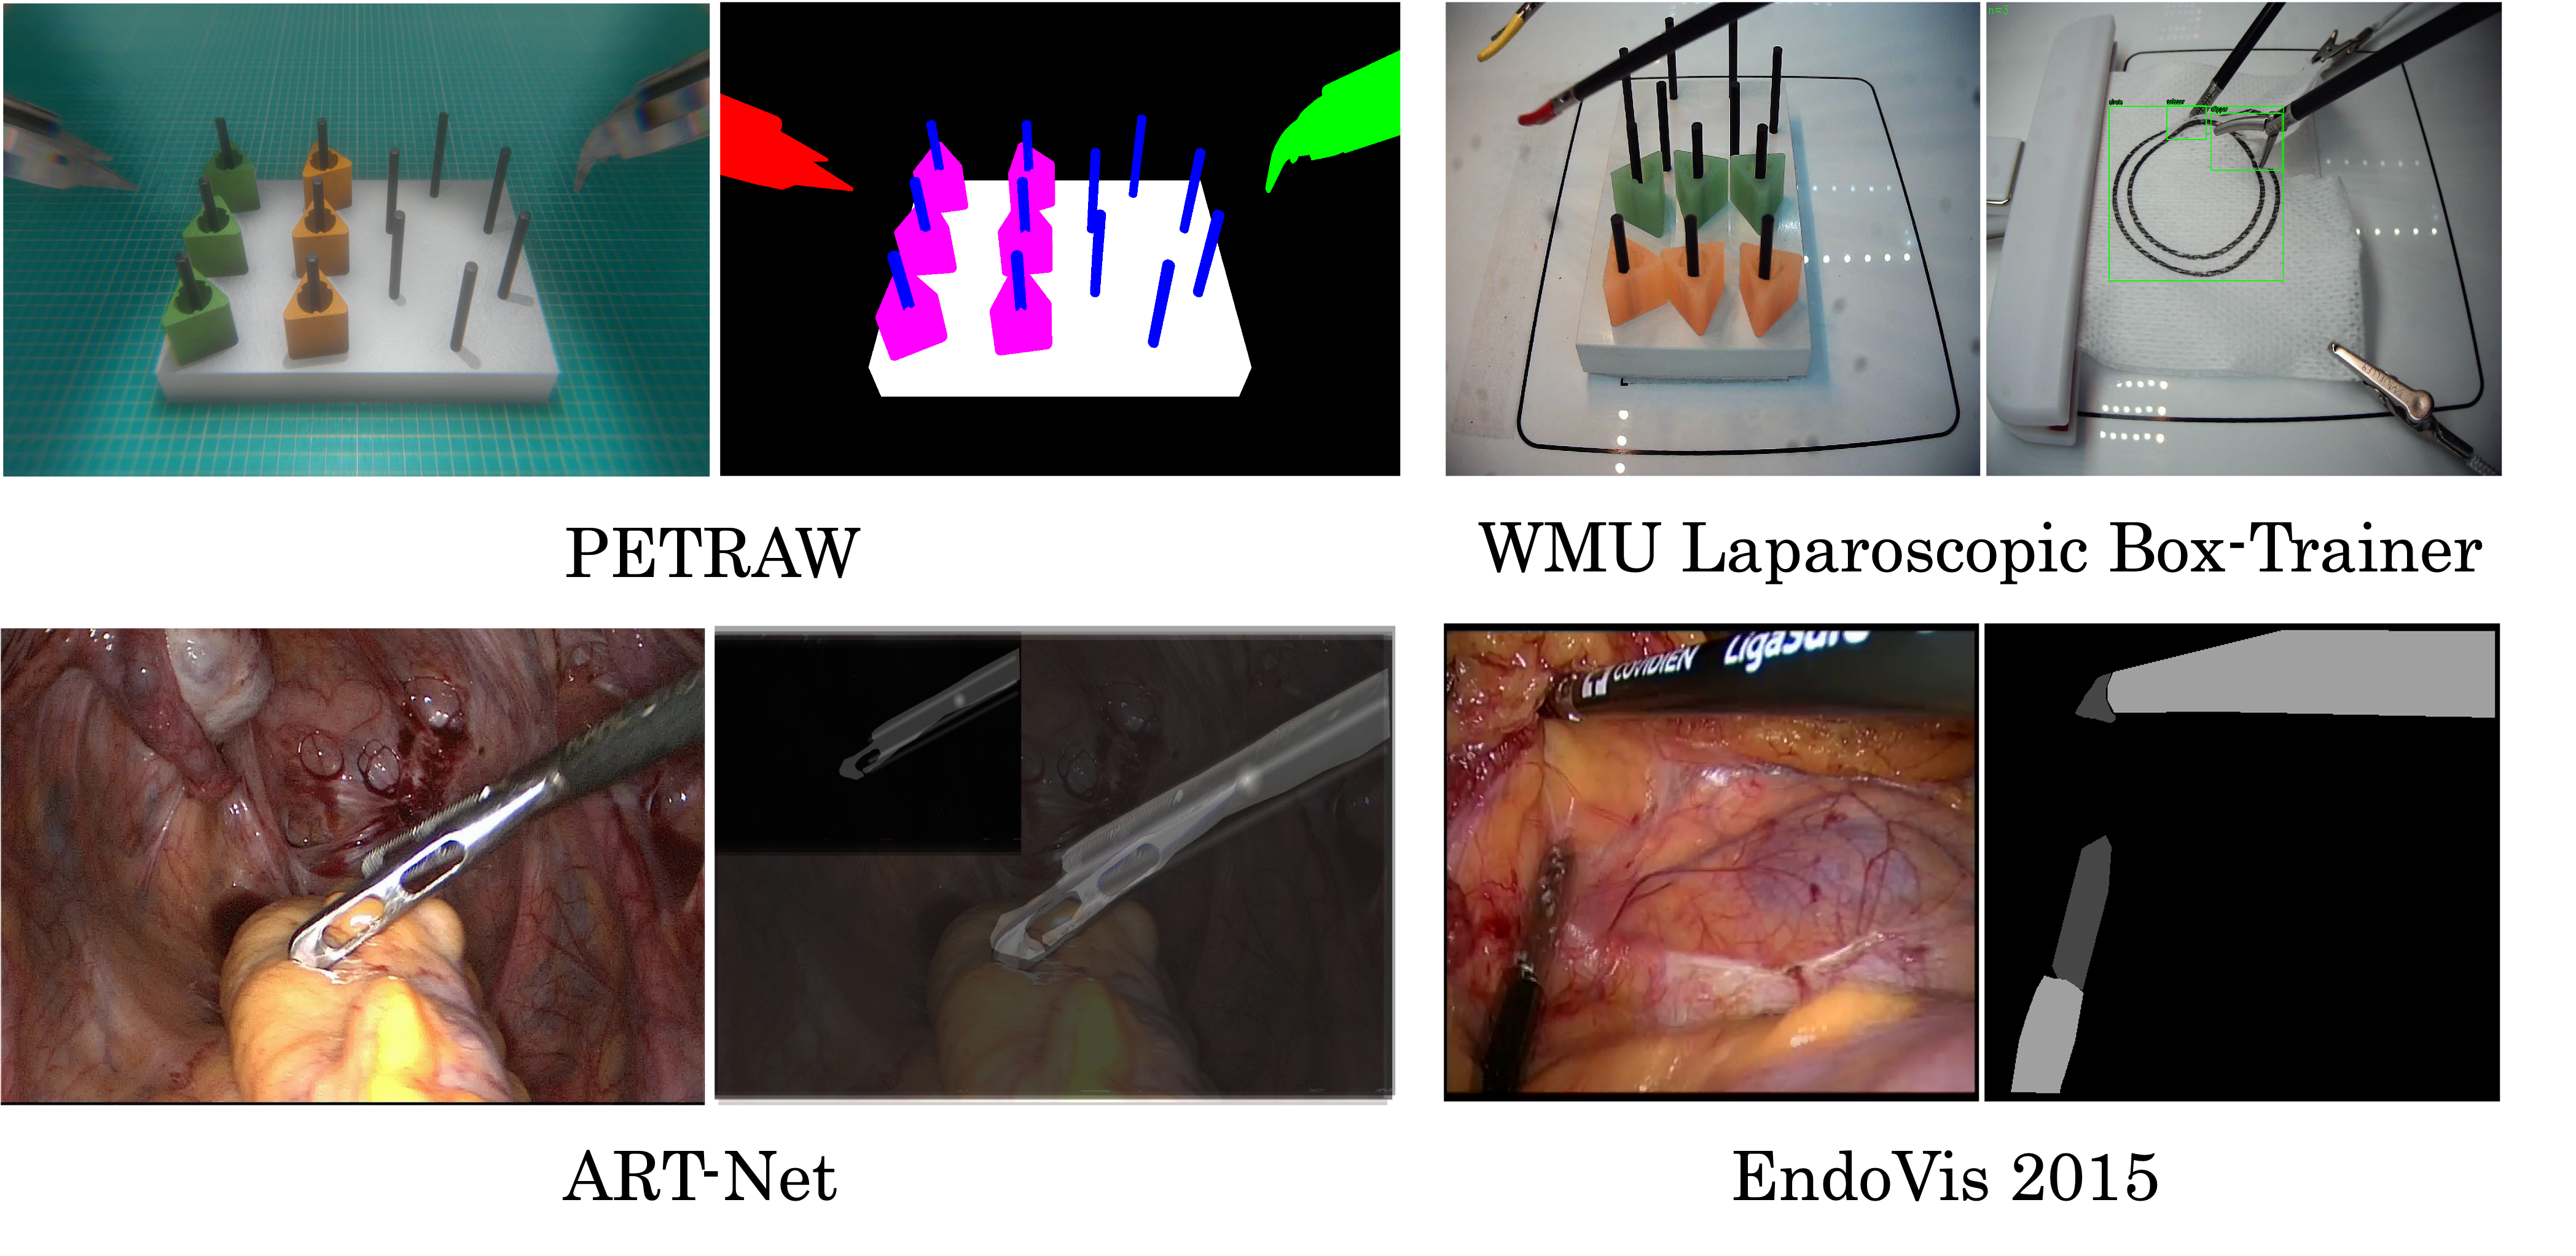
\includegraphics[width=\linewidth]{dataset_samples.png}
    \vspace*{-8mm}
    \caption{Dataset Samples}
    \vspace*{-4mm}
    \label{fig:dataset_samples}
    \Description{Sample dataset images and annotations.}
\end{figure}

Figure \ref{fig:dataset_samples} shows example frames and annotations of some of these datasets. The EndoVis challenge is a high-profile international yearly challenge for the comparative validation of endoscopic vision algorithms \cite{fernandes_future_2023}. The tooltips in EndoVis 2015  are segmentation maps instead of precise points, meaning we can only use them for qualitative analysis. WMU is very similar to AI-ELT; however, it has extremely limited annotations and contains coloured tips, unwantedly simplifying detection \cite{fathabadi_box-trainer_2022}. PETRAW is designed for workflow recognition, comprising 150 sequences of peg transfer sessions recorded on a virtual reality simulator, with available kinematic data, videos, semantic segmentation and workflow annotations, but lacking skill annotations \cite{alabi_multitask_2024, huaulme_peg_2022}. However, detection will be easier since the tools have an almost translucent reflective surface. Using simulated or generated datasets \cite{cartucho_visionblender_2021} will not apply to surgical training LMICs, but they provide the "gold standard" for motion and image annotations. Overall, the ART-Net dataset is the most appropriate as we can compare the models' results, especially those obtained by Hasan directly, assisting in a thorough analysis \cite{hasan_detection_2021}. It is annotated with tool presences (1500 positive cases and 1500 negative cases), tool segmentation maps (635 images), and instrument geometric primitives (mid-line, edge-lines, and precise tooltip points - something valuable most datasets lack).
% ...(mid-line, edge-line, and tooltip, which allow the tool's 3D pose to be estimated by a fast algebraic procedure). Further work has been done on this dataset in segmentation \cite{lou_min-max_2022, rabbani_can_2024}. 
% Surgical datasets can be categorised into specific use cases, e.g. segmentation masks and bounding polygons can be used for segmentation; phase annotations for workflow recognition, ground truth sensor data for pose estimation, classification of the operators' expertise for surgical skill, bounding box annotations can be used for detection, videos and temporal data can be used for tracking  \cite{rodrigues_surgical_2022}. Using a dataset to evaluate implemented object detection methods is essential. However, none of the 64 surgical datasets we initially identified completely fitted our requirements of a multi-class, multi-tool, in-vitro laparoscopic context (even beyond peg-transfer), with skill, bounding box, and motion annotations in a temporal context without markers or artefacts impacting the data quality. Ground truth values for three-dimensional position and orientation were usually unavailable for in-vivo data \cite{allan_toward_2013}. Some datasets had more value as the quality of images and annotations were greater, and very few had code available for direct use. We list these datasets as follows: MICCAI  Endoscopic Vision Challenge 2015 \footnote{Many MICCAI and EndoVis datasets are useful, though not all were readily available.} \cite{bernal_comparative_2017}, PEg TRAnsfer Workflow Recognition by different modalities (PETRAW)\footnote{Sub-challenge as a part of MICCAI 2021} \cite{huaulme_peg_2022} and the Augmented Reality Tool Network (ART-Net) dataset \cite{hasan_detection_2021}. Figure \ref{fig:dataset_samples} shows example frames and annotations of some of these datasets. The EndoVis challenge is a high-profile international challenge for the comparative validation of endoscopic vision algorithms that focus on different problems yearly \cite{fernandes_future_2023}. For qualitative analysis, we can use the videos in the 2015 challenge dataset (EndoVis 2015) to test different cases of tools going in and out of frame, altering appearances with positional and rotational movement. However, we cannot use this dataset for training as the tooltips are defined differently, using the segmentation of the entire tip rather than the exact tooltip point. The images and videos in the WMU Laparoscopic Box-Trainer dataset are very similar to those in AI-ELT; however, they are extremely limited in annotations and contain coloured tips, simplifying detection \cite{fathabadi_box-trainer_2022}. The PETRAW dataset is designed for workflow recognition in peg transfer training sessions \cite{huaulme_peg_2022}. It comprises 150 sequences of peg transfer sessions recorded on a virtual reality simulator, with available kinematic data, videos, and annotations for semantic segmentation (for all objects, tools, and background), phases, steps, and action annotations \cite{alabi_multitask_2024, huaulme_peg_2022}. However, it lacks skill annotations, and detection will be easier since the tools have an almost translucent reflective surface. Using simulated or generated datasets \cite{cartucho_visionblender_2021} will not apply to surgical training LMICs, but they provide the "gold standard" for motion and image annotations.
% MICCAI 2016 Endoscopic Vision Challenge (m2cai16), MICCAI 2024 Endoscopic Vision Challenge (SurgVU)\footnote{Based on the previous 2022 and 2023 challenge versions.} 
% We would have used PETRAW, but the dataset was not originally intended for object detection and tracking, so it would not have been easy to compare its results to those of developed models. Using PETRAW was my idea because of the similarities in the data. I thought it would be decent when evaluated in-house. I could use the segmentation mask to change the colours of the entire image to something more similar to what we have. I could even adapt the tool to make it look more similar to ours. The only problem I see is that the tools look to have reflective surfaces in PETRAW. 

% DIAGRAM TO SHOW SPLIT OF DATASETS

\subsection{Potential Gaps and Insights}

While extensive research exists in surgical tool detection, tracking, and skill assessment, there are few in-vitro laparoscopic training datasets, lest those with suitable quality annotations. Sufficiently annotated training data is crucial for integrating AI into surgery \cite{ali2023comprehensivesurveyrecentdeep}. The performance of AI-based models relies heavily upon data availability, which requires expert annotators for labelling. The poor quality of annotated datasets can be attributed to the lack of success stories in surgery compared to other medical domains \cite{maier-hein_surgical_2022}. This necessitates minimising error by annotating frame-level tools and tooltips \cite{teevno_semi-supervised_2023}. Therefore, we aim to produce high-quality annotated in-vitro datasets, beginning with the AI-ELT dataset. 

The AI-ELT dataset varies considerably from existing datasets, meaning existing conclusions from SOTAs may not hold due to differing domains. For a focused analysis, we will investigate whether anchor-based methods can match or outperform anchor-free methods, how anchor-box optimisation impacts this, how model complexity impacts accuracy and inference time, and why methods perform better or fail at specific tasks. For tracking, we focus on markerless, image-based methods to build generalisable models for in-vitro contexts, where detection and tracking are notably more straightforward than in more complex scenarios that may require more advanced techniques such as machine or deep learning.

% ...specific tasks, and innovate where improvements can be made and mistakes solved, especially under challenging samples such as different tool aspect ratios and sizes and occlusions

% The goal is that we can train an AI system to localise the laparoscopic tools using the image alone. This will help us develop a new training system to give automated feedback on individual sub-skills. In this study, we focus on first detecting the tools, which can then be used with the sensor data to build a model which can predict the tools' motion based on the tool's location in the image.